\documentclass{article}
\usepackage[utf8]{inputenc}
\usepackage[a4paper, total={6.4in, 8.75in}]{geometry}
\usepackage{graphicx}
\usepackage[hidelinks]{hyperref}
\usepackage{float}
\usepackage{xcolor}
\usepackage{amsmath}
\usepackage{pgfplots}
\usepackage{tikz}
\usetikzlibrary{automata,positioning,arrows}
\usetikzlibrary{arrows.meta, shapes.geometric}
\usetikzlibrary{arrows,shapes.gates.logic.US,shapes.gates.logic.IEC,calc}
\tikzstyle{branch}=[fill,shape=circle,minimum size=3pt,inner sep=0pt]
\usepackage[backend=biber,style=authoryear-ibid]{biblatex}
\usepackage{svg}
\usepackage{multicol}
\usepackage{comment}
\usepackage{amsfonts}
%til at fjerne de der tal bag sections uden at den fjerner infholdsfortegnelsen
%\makeatletter
%\renewcommand\@seccntformat[1]{}
%\makeatother
%\newcommand{\tegntæller}[1]{%
%\immediate\write18{texcount -1 -sum -merge -char #1.tex > #1-chars.sum }%
%\input{#1-chars.sum}%
%}
%\tegntæller{main}
\title{vending Machine}
\author{William Laursen}
\date{}
\renewcommand*\contentsname{Indhold}
%\addbibresource{}
\newcommand{\mm}{\textbf}
\newcommand{\dd}{\mathrm{d}}
\begin{document}
\maketitle
\tableofcontents
\newpage

\begin{abstract}
This document presents the design and implementation of a vending machine using Chisel, a hardware description language. The machine is designed to accept coins, display the current sum and price, and release a can when the correct amount is inserted.
\end{abstract}

\section{Intro}
\section{Approach}
\section{Design}
\subsection{FSM Design}

\begin{figure}[H]
\centering
\begin{tikzpicture}[->,>=stealth',node distance=3cm,every state/.style={thick,fill=gray!10},initial text=start]

\node[state,initial](0) {Idle};

\node[state](1)[above right of=0] {$P+2$};
\node[state](2)[below right of=0] {$P+5$};
\node[state](3)[below right of=1] {Check sum};
\node[state](4)[above right of=3] {Releasecan};
\node[state](5)[below right of=3] {Alarm};


\draw 
    (0) edge node[above left] {$c_2c_5'$} (1)
    (0) edge node[below left] {$c_2'c_5$} (2)
    (1) edge[bend left] node[rotate=90,above] {$c_2'c_5b'$} (2)
    (2) edge[bend left] node[rotate=-90,above] {$c_2c_5'b'$} (1)
    (1) edge[loop above] node {$c_2c_5'b'$} (1)
    (2) edge[loop below] node {$c_2'c_5b'$} (2)
    (1) edge node[above] {$b$} (3)
    (2) edge node[below] {$b$} (3)
    (3) edge node[below] {$x$} (4)
    (3) edge node[above] {$x'$} (5)
\end{tikzpicture}
\caption{State diagram for the vending machine FSM.}
\label{fig:fsm}
\end{figure}
Where $b$ is the pressing of buy, in the $P+2$ and $P+5$ states, repectively, $b$ is a "dontcare", therefore it is not labelled. $x$ is rather is the comparator "Check sum" checking if coin amount is grater than the predefined can-price. if $x$ is true it trigges release can, if not Alarm is triggered.
\subsection{Datapath Design}
% Important: If latex complains about unicode characters,
% please use "\usepackage[utf8x]{inputenc}" in your preamble
% You can change the size of the picture by putting it into the construct:
% 1) \resizebox{10cm}{!}{"below picture"} to scale horizontally to 10 cm
% 2) \resizebox{!}{15cm}{"below picture"} to scale vertically to 15 cm
% 3) \resizebox{10cm}{15cm}{"below picture"} a combination of above two
% It is not recomended to use the scale option of the tikzpicture environment.
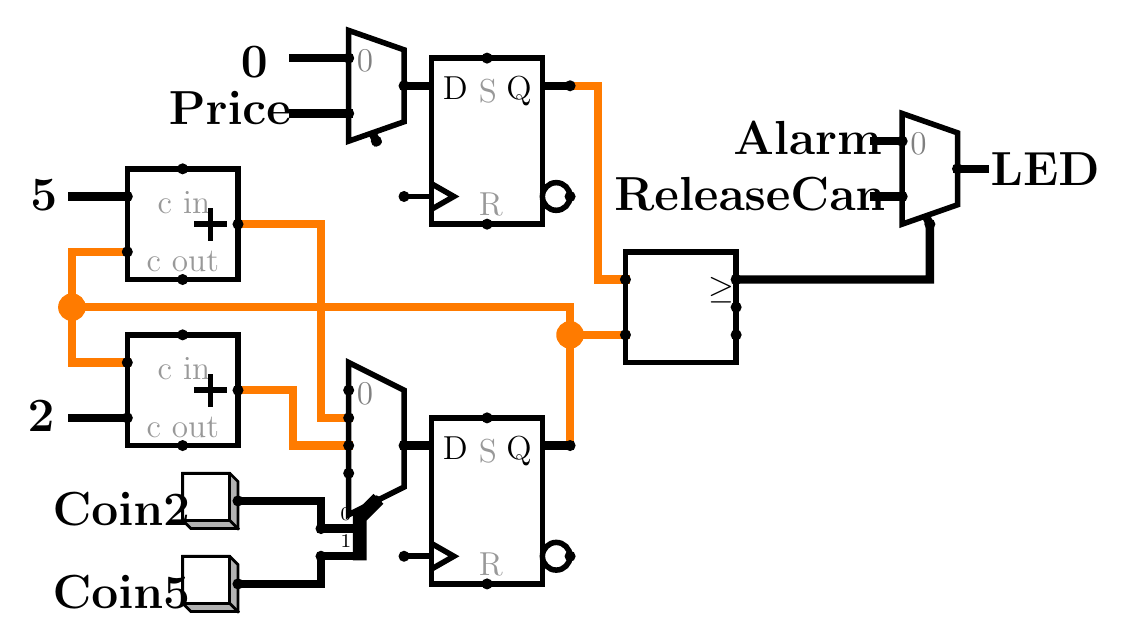
\begin{tikzpicture}[x=1pt,y=-1pt,line cap=rect]
\def\logisimfontA#1{\fontfamily{cmr}{#1}} % Replaced by logisim, original font was "SansSerif"
\definecolor{custcol_FF7B00}{HTML}{FF7B00}
\definecolor{custcol_B2B2B2}{HTML}{B2B2B2}
\definecolor{custcol_FFFFFF}{HTML}{FFFFFF}
\definecolor{custcol_000000}{HTML}{000000}
\definecolor{custcol_999999}{HTML}{999999}
\definecolor{custcol_808080}{HTML}{808080}
\draw [line width=3pt, custcol_FF7B00] (205,120) -- (205,160);
\draw [line width=3pt, custcol_FF7B00] (225,120) -| (205,110) -| (25,90) -- (45,90);
\draw [line width=3pt, custcol_FF7B00] (25,110) |- (45,130);
\draw [line width=3pt, custcol_000000] (25,70) -- (45,70);
\draw [line width=3pt, custcol_000000] (25,150) -- (45,150);
\draw [line width=3pt, custcol_000000] (105,20) -- (125,20);
\draw [line width=3pt, custcol_000000] (105,40) -- (125,40);
\draw [line width=3pt, custcol_FF7B00] (85,140) -| (105,160) -- (125,160);
\draw [line width=3pt, custcol_000000] (315,50) -- (325,50);
\draw [line width=3pt, custcol_000000] (345,60) -- (355,60);
\draw [line width=3pt, custcol_000000] (315,70) -- (325,70);
\draw [line width=3pt, custcol_FF7B00] (85,80) -| (115,150) -- (125,150);
\draw [line width=3pt, custcol_FF7B00] (205,30) -| (215,100) -- (225,100);
\fill [line width=3pt, custcol_FF7B00] (25,110) circle (5);
\fill [line width=3pt, custcol_FF7B00] (205,120) circle (5);
\draw [line width=3pt, custcol_000000] (134,48) -- (135,50);
\logisimfontA{\fontsize{12pt}{12pt}\selectfont\node[inner sep=0, outer sep=0, custcol_808080, anchor=base west] at  (128,25)  {0};}
\draw [line width=2pt, custcol_000000] (125,10) -- (145,17) -- (145,43) -- (125,50) -- cycle;
\fill [line width=2pt, custcol_000000] (125,20) circle (2);
\fill [line width=2pt, custcol_000000] (125,40) circle (2);
\fill [line width=2pt, custcol_000000] (135,50) circle (2);
\logisimfontA{\fontsize{16pt}{16pt}\fontseries{bx}\selectfont\node[inner sep=0, outer sep=0, custcol_000000, anchor=base west] at  (86,27)  {0};}
\logisimfontA{\fontsize{16pt}{16pt}\fontseries{bx}\selectfont\node[inner sep=0, outer sep=0, custcol_000000, anchor=base west] at  (60,44)  {Price};}
\logisimfontA{\fontsize{12pt}{12pt}\selectfont\node[inner sep=0, outer sep=0, custcol_808080, anchor=base west] at  (128,145)  {0};}
\draw [line width=2pt, custcol_000000] (125,130) -- (145,140) -- (145,175) -- (125,185) -- cycle;
\fill [line width=2pt, custcol_000000] (125,140) circle (2);
\fill [line width=2pt, custcol_000000] (125,150) circle (2);
\fill [line width=2pt, custcol_000000] (125,160) circle (2);
\fill [line width=2pt, custcol_000000] (125,170) circle (2);
\fill [line width=1pt, custcol_B2B2B2] (65,200) -- (82,200) -- (85,203) |- (68,220) -- (65,217) -- cycle;
\fill [line width=1pt, custcol_FFFFFF] (65,200) rectangle (82,217);
\draw [line width=1pt, custcol_000000] (65,200) rectangle (82,217);
\draw [line width=1pt, custcol_000000] (82,217) -- (85,220);
\draw [line width=1pt, custcol_000000] (65,200) -- (82,200) -- (85,203) |- (68,220) -- (65,217) -- cycle;
\logisimfontA{\fontsize{16pt}{16pt}\fontseries{bx}\selectfont\node[inner sep=0, outer sep=0, custcol_000000, anchor=base west] at  (18,219)  {Coin5};}
\fill [line width=1pt, custcol_000000] (85,210) circle (2);
\fill [line width=1pt, custcol_B2B2B2] (65,170) -- (82,170) -- (85,173) |- (68,190) -- (65,187) -- cycle;
\fill [line width=1pt, custcol_FFFFFF] (65,170) rectangle (82,187);
\draw [line width=1pt, custcol_000000] (65,170) rectangle (82,187);
\draw [line width=1pt, custcol_000000] (82,187) -- (85,190);
\draw [line width=1pt, custcol_000000] (65,170) -- (82,170) -- (85,173) |- (68,190) -- (65,187) -- cycle;
\logisimfontA{\fontsize{16pt}{16pt}\fontseries{bx}\selectfont\node[inner sep=0, outer sep=0, custcol_000000, anchor=base west] at  (18,189)  {Coin2};}
\fill [line width=1pt, custcol_000000] (85,180) circle (2);
\draw [line width=3pt, custcol_000000] (85,180) -| (115,190) -- (129,190);
\draw [line width=3pt, custcol_000000] (85,210) -| (115,200) -- (129,200);
\draw [line width=5pt, custcol_000000] (129,199) -- (129,186) -- (134,181);
\logisimfontA{\fontsize{7pt}{7pt}\selectfont\node[inner sep=0, outer sep=0, custcol_000000, anchor=base west] at  (122,187)  {0};}
\logisimfontA{\fontsize{7pt}{7pt}\selectfont\node[inner sep=0, outer sep=0, custcol_000000, anchor=base west] at  (122,197)  {1};}
\fill [line width=5pt, custcol_000000] (135,180) circle (2);
\fill [line width=5pt, custcol_000000] (115,190) circle (2);
\fill [line width=5pt, custcol_000000] (115,200) circle (2);
\draw [line width=2pt, custcol_000000] (45,60) rectangle (85,100);
\fill [line width=1pt, custcol_000000] (45,70) circle (2);
\fill [line width=1pt, custcol_000000] (45,90) circle (2);
\fill [line width=1pt, custcol_000000] (85,80) circle (2);
\fill [line width=1pt, custcol_000000] (65,60) circle (2);
\logisimfontA{\fontsize{12pt}{12pt}\selectfont\node[inner sep=0, outer sep=0, custcol_999999, anchor=base west] at  (56,76)  {c in};}
\fill [line width=1pt, custcol_000000] (65,100) circle (2);
\logisimfontA{\fontsize{12pt}{12pt}\selectfont\node[inner sep=0, outer sep=0, custcol_999999, anchor=base west] at  (52,97)  {c out};}
\draw [line width=2pt, custcol_000000] (70,80) -- (80,80);
\draw [line width=2pt, custcol_000000] (75,75) -- (75,85);
\draw [line width=2pt, custcol_000000] (45,120) rectangle (85,160);
\fill [line width=1pt, custcol_000000] (45,130) circle (2);
\fill [line width=1pt, custcol_000000] (45,150) circle (2);
\fill [line width=1pt, custcol_000000] (85,140) circle (2);
\fill [line width=1pt, custcol_000000] (65,120) circle (2);
\logisimfontA{\fontsize{12pt}{12pt}\selectfont\node[inner sep=0, outer sep=0, custcol_999999, anchor=base west] at  (56,136)  {c in};}
\fill [line width=1pt, custcol_000000] (65,160) circle (2);
\logisimfontA{\fontsize{12pt}{12pt}\selectfont\node[inner sep=0, outer sep=0, custcol_999999, anchor=base west] at  (52,157)  {c out};}
\draw [line width=2pt, custcol_000000] (70,140) -- (80,140);
\draw [line width=2pt, custcol_000000] (75,135) -- (75,145);
\logisimfontA{\fontsize{16pt}{16pt}\fontseries{bx}\selectfont\node[inner sep=0, outer sep=0, custcol_000000, anchor=base west] at  (10,75)  {5};}
\logisimfontA{\fontsize{16pt}{16pt}\fontseries{bx}\selectfont\node[inner sep=0, outer sep=0, custcol_000000, anchor=base west] at  (9,155)  {2};}
\draw [line width=2pt, custcol_000000] (155,150) rectangle (195,210);
\fill [line width=2pt, custcol_000000] (175,210) circle (2);
\logisimfontA{\fontsize{12pt}{12pt}\selectfont\node[inner sep=0, outer sep=0, custcol_999999, anchor=base west] at  (172,207)  {R};}
\fill [line width=2pt, custcol_000000] (175,150) circle (2);
\logisimfontA{\fontsize{12pt}{12pt}\selectfont\node[inner sep=0, outer sep=0, custcol_999999, anchor=base west] at  (172,166)  {S};}
\draw [line width=3pt, custcol_000000] (145,160) -- (154,160);
\fill [line width=3pt, custcol_000000] (145,160) circle (2);
\logisimfontA{\fontsize{12pt}{12pt}\selectfont\node[inner sep=0, outer sep=0, custcol_000000, anchor=base west] at  (159,165)  {D};}
\draw [line width=2pt, custcol_000000] (156,196) -- (163,200) -- (156,204);
\draw [line width=2pt, custcol_000000] (145,200) -- (154,200);
\fill [line width=2pt, custcol_000000] (145,200) circle (2);
\draw [line width=3pt, custcol_000000] (196,160) -- (205,160);
\logisimfontA{\fontsize{12pt}{12pt}\selectfont\node[inner sep=0, outer sep=0, custcol_000000, anchor=base west] at  (182,165)  {Q};}
\fill [line width=3pt, custcol_000000] (205,160) circle (2);
\draw [line width=2pt, custcol_000000] (200,200) circle (5);
\fill [line width=2pt, custcol_000000] (205,200) circle (2);
\draw [line width=2pt, custcol_000000] (155,20) rectangle (195,80);
\fill [line width=2pt, custcol_000000] (175,80) circle (2);
\logisimfontA{\fontsize{12pt}{12pt}\selectfont\node[inner sep=0, outer sep=0, custcol_999999, anchor=base west] at  (172,77)  {R};}
\fill [line width=2pt, custcol_000000] (175,20) circle (2);
\logisimfontA{\fontsize{12pt}{12pt}\selectfont\node[inner sep=0, outer sep=0, custcol_999999, anchor=base west] at  (172,36)  {S};}
\draw [line width=3pt, custcol_000000] (145,30) -- (154,30);
\fill [line width=3pt, custcol_000000] (145,30) circle (2);
\logisimfontA{\fontsize{12pt}{12pt}\selectfont\node[inner sep=0, outer sep=0, custcol_000000, anchor=base west] at  (159,35)  {D};}
\draw [line width=2pt, custcol_000000] (156,66) -- (163,70) -- (156,74);
\draw [line width=2pt, custcol_000000] (145,70) -- (154,70);
\fill [line width=2pt, custcol_000000] (145,70) circle (2);
\draw [line width=3pt, custcol_000000] (196,30) -- (205,30);
\logisimfontA{\fontsize{12pt}{12pt}\selectfont\node[inner sep=0, outer sep=0, custcol_000000, anchor=base west] at  (182,35)  {Q};}
\fill [line width=3pt, custcol_000000] (205,30) circle (2);
\draw [line width=2pt, custcol_000000] (200,70) circle (5);
\fill [line width=2pt, custcol_000000] (205,70) circle (2);
\draw [line width=3pt, custcol_000000] (334,78) -- (335,80) |- (265,100);
\logisimfontA{\fontsize{12pt}{12pt}\selectfont\node[inner sep=0, outer sep=0, custcol_808080, anchor=base west] at  (328,55)  {0};}
\draw [line width=2pt, custcol_000000] (325,40) -- (345,47) -- (345,73) -- (325,80) -- cycle;
\fill [line width=2pt, custcol_000000] (325,50) circle (2);
\fill [line width=2pt, custcol_000000] (325,70) circle (2);
\fill [line width=2pt, custcol_000000] (335,80) circle (2);
\fill [line width=2pt, custcol_000000] (345,60) circle (2);
\logisimfontA{\fontsize{16pt}{16pt}\fontseries{bx}\selectfont\node[inner sep=0, outer sep=0, custcol_000000, anchor=base west] at  (357,66)  {LED};}
\logisimfontA{\fontsize{16pt}{16pt}\fontseries{bx}\selectfont\node[inner sep=0, outer sep=0, custcol_000000, anchor=base west] at  (221,75)  {ReleaseCan};}
\logisimfontA{\fontsize{16pt}{16pt}\fontseries{bx}\selectfont\node[inner sep=0, outer sep=0, custcol_000000, anchor=base west] at  (264,55)  {Alarm};}
\draw [line width=2pt, custcol_000000] (225,90) rectangle (265,130);
\fill [line width=1pt, custcol_000000] (225,100) circle (2);
\fill [line width=1pt, custcol_000000] (225,120) circle (2);
\fill [line width=1pt, custcol_000000] (265,100) circle (2);
\logisimfontA{\fontsize{12pt}{12pt}\selectfont\node[inner sep=0, outer sep=0, custcol_000000, anchor=base west] at  (255,107)  {$\geq$};}
\fill [line width=1pt, custcol_000000] (265,110) circle (2);
\logisimfontA{\fontsize{12pt}{12pt}\selectfont\node[inner sep=0, outer sep=0, custcol_000000, anchor=base west] at  (255,117)  { };}
\fill [line width=1pt, custcol_000000] (265,120) circle (2);
\logisimfontA{\fontsize{12pt}{12pt}\selectfont\node[inner sep=0, outer sep=0, custcol_000000, anchor=base west] at  (255,127)  { };}
\end{tikzpicture}

\section{Implementation}
\section{Results}
\section{Discussion}
\subsection{Reflection on using AI}

%the abstract is written by AI 
\section{Conclusion}

\appendix
\section{code}
\section{test video}
\begin{figure}[H]
\centering

\includegraphics[angle=0]{./testvideoqr.eps}
\caption{Video of test on Basys3 board}
\label{videotestofprod}
\end{figure}


%\printbibliography[heading=none]
\end{document}